%%%%%%%%%%%%%%%%%%%%%%%%%%%%%%%%%%%%%%%%%%%%%%%%%%%%%%%%%%%%%%%%%%%%%%%%%%%%%%%%
%%%%%%%%%%%%%%%%%%%%%%%%%%%%%%%%%%%%%%%%%%%%%%%%%%%%%%%%%%%%%%%%%%%%%%%%%%%%%%%%
%
% A general frame for lecture slides and lecture notes in one file
% using LaTeX beamer
%
%%%%%%%%%%%%%%%%%%%%%%%%%%%%%%%%%%%%%%%%%%%%%%%%%%%%%%%%%%%%%%%%%%%%%%%%%%%%%%%%
%%%%%%%%%%%%%%%%%%%%%%%%%%%%%%%%%%%%%%%%%%%%%%%%%%%%%%%%%%%%%%%%%%%%%%%%%%%%%%%%
\documentclass[ignorenonframetext,11pt]{beamer}
%\usepackage[ngerman]{babel}
%\usepackage[T1]{fontenc}
\usepackage[utf8]{inputenc}
\usepackage{lmodern}
\usepackage{amsmath,amssymb,amsfonts}


% only presentation 
\mode<presentation>
{
  \usetheme{default}
%  \usecolortheme{crane}
  \setbeamercovered{transparent}
%  \setlength{\parindent}{0pt}
%  \setlength{\parskip}{1.35ex plus 0.5ex minus 0.3ex}
%  \usefonttheme{structuresmallcapsserif}
  \usefonttheme{structurebold}
  \setbeamertemplate{theorems}[numbered]
  \usepackage{amscd}
}

% all after
\usepackage{tikz} 
\usepackage{pgfplots,adjustbox}
\usepackage{eurosym} 
\usepackage{graphicx}
\usepackage{multimedia}
\usepackage{psfrag}
\usepackage{listings}
\lstset{language=C++, basicstyle=\ttfamily, 
  keywordstyle=\color{black}\bfseries, tabsize=4, stringstyle=\ttfamily,
  commentstyle=\it, extendedchars=true, escapeinside={/*@}{@*/}}
\usepackage{curves}
%\usepackage{epic}
\usepackage{calc}
%\usepackage{picinpar}
%\usepackage{fancybox}
%\usepackage{xspace}
\usepackage{enumerate}
\usepackage{algpseudocode}
\usepackage{color}
\usepackage{bold-extra}
\usepackage{bm}
\usepackage{stmaryrd}
%\usepackage[squaren]{SIunits}
\usepackage{nicefrac}

\usepackage{fancyvrb,bbm,xspace}
\usepackage{lmodern}
\usepackage{fancyvrb,bbm,xspace}
\usepackage[binary-units]{siunitx}
\usepackage{xcolor,tabu}

\definecolor{niceblue}{rgb}{0.122,0.396,0.651}   %% 31, 101, 166 or #1F65A6
\definecolor{niceorange}{RGB}{255,205,86}        %% #FFCD56
\definecolor{nicered}{RGB}{220,20,60}                      %% rgb(220, 20, 60)
\definecolor{niceteal}{HTML}{00A9AB}
\definecolor{niceviolet}{HTML}{820080}

\definecolor{niceblueLight}{HTML}{91CAFB}
\definecolor{niceblueVeryLight}{HTML}{DDEFFF}

\usepackage{dsfont}

%\newcommand{\hlineabove}{\rule{0pt}{2.6ex}}
%\newcommand{\hlinebelow}{\rule[-1.2ex]{0pt}{0pt}}

%\usecolortheme[RGB={37,75,123}]{structure}
% \definecolor{structurecolor}{rgb}{0.905,0.318,0.071}

% \setbeamercolor{frametitle}{fg=black,bg=}
% \setbeamercolor{sidebar left}{fg=,bg=}

% \setbeamertemplate{headline}{\vskip4em}
% \setbeamersize{sidebar width left=.9cm}

% \setbeamertemplate{navigation symbols}{}
%\setbeamertemplate{blocks}[rounded][shadow=true]
%\setbeamertemplate{itemize items}[square]

\mode<presentation> 
{
\theoremstyle{definition}
}
\newtheorem{Def}{Definition}%[section]
\newtheorem{Exm}[Def]{Example}
\newtheorem{Lem}[Def]{Lemma}
\newtheorem{Rem}[Def]{Remark}
\newtheorem{Rul}[Def]{Rule}
\newtheorem{Thm}[Def]{Theorem}
\newtheorem{Cor}[Def]{Corollary}
\newtheorem{Obs}[Def]{Observation}
\newtheorem{Ass}[Def]{Assumption}
\newtheorem{Pro}[Def]{Property}
\newtheorem{Alg}[Def]{Algorithm}
\newtheorem{Prp}[Def]{Proposition}
\newtheorem{Lst}[Def]{Listing}

% Delete this, if you do not want the table of contents to pop up at
% the beginning of each subsection:
\AtBeginSection[]
{
  \begin{frame}<beamer>
    \frametitle{Contents}
    \tableofcontents[sectionstyle=show/shaded,subsectionstyle=hide/hide/hide]
%\tableofcontents[currentsection]
  \end{frame}
}

% Title definition
\mode<presentation>
{
  \title{DUNE PDELab Tutorial 05\\
  {\small  Adaptivity in PDELab}}
  \author{Ole Klein}
  \institute[]
  {
   Interdisziplinäres Zentrum für Wissenschaftliches Rechnen\\
   Im Neuenheimer Feld 205, D-69120 Heidelberg \\[6pt]
  }
  \date[\today]{\today}
}


% logo nach oben
\mode<presentation>
{
% No navigation symbols and no lower logo
\setbeamertemplate{sidebar right}{}

% logo
\newsavebox{\logobox}
\sbox{\logobox}{%
    \hskip\paperwidth%
    \rlap{%
      % putting the logo should not change the vertical possition
      \vbox to 0pt{%
        \vskip-\paperheight%
        \vskip0.35cm%
        \llap{\insertlogo\hskip0.1cm}%
        % avoid overfull \vbox messages
        \vss%
      }%
    }%
}

\addtobeamertemplate{footline}{}{%
    \usebox{\logobox}%
}
}

%%%%%%%%%%%%%%%%%%%%%%%%%%%%%%%%%%%%%%%%%%%%%%%%%%%%%%%%%%%%%%%%%%%%%%%%%%%%%%%%
%%%%%%%%%%%%%%%%%%%%%%%%%%%%%%%%%%%%%%%%%%%%%%%%%%%%%%%%%%%%%%%%%%%%%%%%%%%%%%%%
%
% now comes the individual stuff lecture by lecture
%
%%%%%%%%%%%%%%%%%%%%%%%%%%%%%%%%%%%%%%%%%%%%%%%%%%%%%%%%%%%%%%%%%%%%%%%%%%%%%%%%
%%%%%%%%%%%%%%%%%%%%%%%%%%%%%%%%%%%%%%%%%%%%%%%%%%%%%%%%%%%%%%%%%%%%%%%%%%%%%%%%

\begin{document}

\frame{\titlepage}

%%%%%%%%%%%%%%%%%%%%%%%%%%%%%%%%%%%%%%%%%%%%%%%%%%%%%%%%%%%%%%%%%%%%%%%%%%%%%%%%
%%%%%%%%%%%%%%%%%%%%%%%%%%%%%%%%%%%%%%%%%%%%%%%%%%%%%%%%%%%%%%%%%%%%%%%%%%%%%%%%

\begin{frame}
\frametitle{Motivation}
\begin{itemize}
  \item Provide a comparatively simple example of adaptive mesh refinement in
    PDELab
  \item Build upon problem definition that is already familiar (tutorial 01)
  \item Integrate central steps into framework that was introduced for the
    solution of PDEs
  \item Show where the approach could be extended and modified to suit other PDEs,
    error norms or performance functionals
\end{itemize}
\end{frame}

\begin{frame}
\frametitle{Discretization Error}
\begin{itemize}
  \item FEM approach replaces solution space $V$, e.g. $V=H^1(\Omega)$ plus
    constraints, with \emph{finite-dimensional} space $V_h$
  \item FEM solution $u_h \in V_h$ is approximation of solution $u \in V$
  \item Finite approximation leads to discretization error, which should be small:
    \begin{equation*}
      \| u - u_h \| \leq \text{TOL}
    \end{equation*}
  \item $\| \cdot \|$ is suitable norm, e.g. $L^2$ or $H^1$ norm, $\text{TOL}$ is
    user-supplied tolerance
\end{itemize}
\end{frame}

\begin{frame}
\frametitle{Central Aspects of Mesh Generation}
\begin{itemize}
  \item Number of degrees of freedom (dofs) important for applicability of method:
    \begin{itemize}
      \item Directly translates to memory requirements
      \item Determines computation time (together with mesh geometry)
    \end{itemize}
  \item Keep number of dofs as small as possible while fulfilling requirements for
    error norm $\| u - u_h \|$
  \item Discretization error $u - u_h$ is generally not known (else there would be
    no need for FEM!)
  \item A-priori error estimates are for worst case, i.e. may be overly pessimistic,
    don't provide spatially resolved information and contain unknown constant
\end{itemize}
$\Rightarrow$ \emph{A-posteriori error estimates} and iterative procedure required
\end{frame}

\begin{frame}
\begin{center}
\Large\textbf{Derivation of Local Error Indicators}
\end{center}
\end{frame}

%%%%%%%%%%%%%%%%%%%%%%%%%%%%%%%%%%%%%%%%%%%%%%%%%%%%%%%%%%%%%%%%%%%%%%%%%%%%%%%%
%%%%%%%%%%%%%%%%%%%%%%%%%%%%%%%%%%%%%%%%%%%%%%%%%%%%%%%%%%%%%%%%%%%%%%%%%%%%%%%%

\begin{frame}
\frametitle{PDE Problem}
We consider the problem
\begin{subequations} \label{eq:ProblemStrong}
\begin{align*}
-\Delta u + q(u) &= f &&\text{in $\Omega$},\\
u &= g &&\text{on $\Gamma_D\subseteq\partial\Omega$},\\
-\nabla u\cdot \nu &= j &&\text{on $\Gamma_N=\partial\Omega\setminus\Gamma_D$}.
\end{align*}
\end{subequations}
\begin{itemize}
\item $q:\mathbb{R}\to\mathbb{R}$ is possibly
nonlinear function
\item $f: \Omega\to\mathbb{R}$ the source term
\item $\nu$ unit outer normal to the domain
\end{itemize}
\end{frame}

\begin{frame}
\frametitle{Weak Formulation}
\begin{equation*}
\text{Find $u\in U$ s.t.:} \quad r^{\text{NLP}}(u,v)=0 \quad \forall v\in V,
\end{equation*}
with the continuous residual form
\begin{equation*}
r^{\text{NLP}}(u,v) = \int_\Omega \nabla u \cdot \nabla v + (q(u)-f)v\,dx + \int_{\Gamma_N} jv\,ds
\end{equation*}
and the function spaces 
\begin{itemize}
\item $U= \{v\in H^1(\Omega) \,:\, \text{``$v=g$'' on $\Gamma_D$}\}$ (affine space)
\item $V= \{v\in H^1(\Omega) \,:\, \text{``$v=0$'' on $\Gamma_D$}\}$
\end{itemize}
We assume that a unique solution exists.
\end{frame}

\begin{frame}
\frametitle{For Derivation: Linear PDE Problem}
The presented derivation of local error estimates requires that the PDE is linear.
We therefore consider
\begin{equation*}
\text{Find $u\in U$ s.t.:} \quad r^{\text{LP}}(u,v)=0 \quad \forall v\in V,
\label{Eq:BasicBuildingBlock}
\end{equation*}
with the continuous residual form
\begin{equation*}
  r^{\text{LP}}(u,v) = \int_\Omega \nabla u \cdot \nabla v + (cu-\tilde{f})v\,dx + \int_{\Gamma_N} jv\,ds
\end{equation*}
i.e. $q(u) = c u$ with a constant $c \in \mathbb{R}$ and a different right hand
side $\tilde{f}$, and later return to the original nonlinear PDE.
\end{frame}

\begin{frame}
\frametitle{Discretization Error Identity}
Define \emph{discretization error} $e = u - u_h \in V$ and bilinear form
\begin{equation*}
  a(u,v) = \int_\Omega \nabla u \cdot \nabla v + c u v \,dx
\end{equation*}
Then we have, due to linearity of the PDE,
\begin{align*}
  a(e,v) &= a(u,v) - a(u_h,v) \\
  &= r^{LP}(u,v) - r^{LP}(u_h,v) \\
  &= - r^{LP}(u_h,v)
\end{align*}
This provides an expression that does not depend on $u$ and therefore can be
evaluated using the finite element solution $u_h$!
\end{frame}

\begin{frame}
\frametitle{Element Residuals}
\begin{align*}
  a(e,v) &= - r^{LP}(u_h,v) \\
  &= - \int_\Omega \nabla u_h \cdot \nabla v + (c u_h - \tilde{f})\,dx - \int_{\Gamma_N} jv\,ds \\
  &= - \sum_{T \in \mathcal{T}_h} \left\{ \int_T \nabla u_h \cdot \nabla v + (c u_h - \tilde{f})\,dx - \int_{\partial T \cap \Gamma_N} jv\,ds \right\} \\
  &= \sum_{T \in \mathcal{T}_h} \left\{ \int_T R_T v \,dx + \int_{\partial T} R_{\partial T} v \,ds \right\}
\end{align*}
with \emph{element residuals} $R_T$ and \emph{element boundary residuals} $R_{\partial T}$ given by
\begin{align*}
  R_T &= \Delta u_h + \tilde{f} - c u_h \\
  R_{\partial T} &= \begin{cases} - (\nabla u_h) \cdot \nu & \text{on } \partial T \setminus \Gamma_N \\
    -(\nabla u_h) \cdot \nu - j & \text{on } \partial T \cap \Gamma_N \end{cases}
\end{align*}
\end{frame}

\begin{frame}
\frametitle{Face Residuals}
There are three types of faces $F \in \mathcal{F}_h$ that contribute to $\partial T$:
\begin{itemize}
  \item Interior faces $F \in \mathcal{F}_h^i$, these appear twice in the summation with changing orientation
  \item Neumann boundary faces $F \in \mathcal{F}_h^N$, these appear once
  \item Dirichlet boundary faces $F \in \mathcal{F}_h^D$, here $v$ is zero
\end{itemize}

Define the \emph{face residuals} $R_F$ for faces $F \in \mathcal{F}$ by setting
\begin{equation*}
  R_F = \begin{cases} R_{\partial T}(T^-) + R_{\partial T}(T^+) = [- (\nabla u_h) \cdot \nu_F] & F \in \mathcal{F}_h^i \\
    R_{\partial T}(T^-) = - (\nabla u_h) \cdot \nu_F - j & F \in \mathcal{F}_h^N \end{cases}
\end{equation*}
where $T^-$ and $T^+$ are the elements next to $F$, $\nu_F$ points from $T^-$ to $T^+$ and $[\cdot]$ is the jump operator for tw-valued functions on $F$, i.e.
\begin{equation*}
  [v] = v(T^-) - v(T^+)
\end{equation*}
\end{frame}

\begin{frame}
\frametitle{Discretization Error Identity (cont.)}
Using the element residuals $R_T$ and face residuals $R_F$, we have
\begin{equation*}
  a(e,v) = \sum_{T \in \mathcal{T}_h} \int_T R_T v \,dx + \sum_{F \in \mathcal{F}_h^i \cup \mathcal{F}_h^N} \int_F R_F v \,ds
\end{equation*}

For any interpolation operator $\mathcal{I} \colon V \to V_h$ we also have
\begin{equation*}
  a(e,\mathcal{I}v) = \sum_{T \in \mathcal{T}_h} \int_T R_T \mathcal{I} v \,dx + \sum_{F \in \mathcal{F}_h^i \cup \mathcal{F}_h^N} \int_F R_F \mathcal{I} v \,ds = 0
\end{equation*}
($u_h$ is discrete solution!), and therefore
\begin{equation*}
  a(e,v) = \sum_{T \in \mathcal{T}_h} \int_T R_T (v - \mathcal{I} v) \,dx + \sum_{F \in \mathcal{F}_h^i \cup \mathcal{F}_h^N} \int_F R_F (v - \mathcal{I} v) \,ds
\end{equation*}
\end{frame}

\begin{frame}
\frametitle{Discretization Error Identity (cont.)}
Using
\begin{itemize}
  \item A specific choice of interpolation operator
  \item Matching interpolation error estimates (independent of problem definition!)
  \item Shape regularity of the finite element mesh
\end{itemize}
one can show that
\begin{align*}
  a(e,v) &= \sum_{T \in \mathcal{T}_h} \int_T R_T (v - \mathcal{I} v) \,dx + \sum_{F \in \mathcal{F}_h^i \cup \mathcal{F}_h^N} R_F (v - \mathcal{I} v) \,ds \\
  &\leq C \| v \|_{1,\Omega} \left\{ \sum_{T \in \mathcal{T}_h} h_T^2 \|R_T\|_{0,T}^2 + \sum_{F \in \mathcal{F}_h^i \cup \mathcal{F}_h^N} h_F \| R_F \|_{0,F}^2 \right\}^{1/2}
\end{align*}
\end{frame}

\begin{frame}
\frametitle{Error Estimate}
Set $v = e \in V$ and exploit coercivity $\|e\|_{1,\Omega}^2 \leq C a(e,e)$, then
\begin{align*}
  \|e\|_{1,\Omega} &\leq C \left\{ \sum_{T \in \mathcal{T}_h} h_T^2 \|R_T\|_{0,T}^2 + \sum_{F \in \mathcal{F}_h^i \cup \mathcal{F}_h^N} h_F \|R_F\|_{0,F}^2 \right\}^{1/2} \\
  &\leq C \left\{ \sum_{T \in \mathcal{T}_h} \gamma_T^2 \right\}^{1/2}
\end{align*}
with the \emph{local error indicators}
\begin{equation*}
  \gamma_T^2 = h_T^2 \|R_T\|_{0,T}^2 + \sum_{F \in \partial T \cap \mathcal{F}_h^N} h_T \|R_F\|_{0,F}^2 + \sum_{F \in \partial T \cap \mathcal{F}_h^i} \frac{h_T}{2} \|R_F\|_{0,F}^2
\end{equation*}
\end{frame}

\begin{frame}
\frametitle{Return to nonlinear PDE problem}
For the original nonlinear PDE, linearize residual form around $\xi \in V_h$ and set
\begin{equation*}
  c = \frac{\partial q}{\partial u} |_\xi, \quad \tilde{f} = f - q(\xi) + \frac{\partial q}{\partial u} |_\xi \xi
\end{equation*}
The choice $\xi = u_h$ provides face residuals as before and element residuals
\begin{equation*}
  R_T = \Delta u_h + f - q(u_h)
\end{equation*}
This can be used to compute local error indicators, but the error inequality only
holds if $u_h$ is sufficiently close to $u$!
\end{frame}

\begin{frame}
\begin{center}
\Large\textbf{Local Mesh Adaptation}
\end{center}
\end{frame}

\begin{frame}
\frametitle{Basic Adaptation Algorithm}
The basic algorithm works as follows:
\begin{enumerate}
  \item Choose sufficiently fine starting mesh $\mathcal{T}_0$
  \item Compute finite element solution $u_h$ on current mesh $\mathcal{T}_h$
  \item Compute error estimate $\gamma(u_h)$, stop if $\gamma(u_h) \leq \text{TOL}$
  \item Else refine mesh according to the local error indicators $\gamma_T$
  \item Transfer current solution $u_h$ and use as initial guess
  \item Go to step 2)
\end{enumerate}
\end{frame}

\begin{frame}
\frametitle{Bulk Fraction Strategy}
\begin{itemize}
  \item Step 4) requires picking elements for refinement
  \item Assumption: spatial distribution of error is similar to that of
    assembled residuals $R_T$ and $R_F$ (reasonable for diffusion-type
    problems)
  \item Sort elements according to increasing error contribution:
    \begin{equation*}
      \gamma_{T_1}^2 \leq \gamma_{T_2}^2 \leq \dots \leq \gamma_{T_N}^2
    \end{equation*}
  \item For given $\rho \in (0,1]$, determine
    \begin{equation*}
      J = \max \left\{ j \colon \sum_{k=j}^N \gamma_{T_k}^2 \geq \rho \sum_{T \in \mathcal{T}_h} \gamma_T^2 \right\}
    \end{equation*}
    and refine elements $T_J,\dots,T_N$
\end{itemize}
\end{frame}

\begin{frame}
\frametitle{Bisection Refinement}
\begin{center}
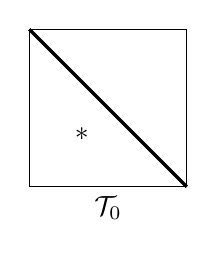
\begin{tikzpicture}[scale=0.5]
\draw (0,0)--(4,0)--(4,4)--(0,4)--(0,0);
\draw[very thick] (0,4)--(4,0);
\node at (1.33,1.33) {$\ast$};
\node[below] at (2,0) {$\mathcal{T}_0$};
\end{tikzpicture} \hfill
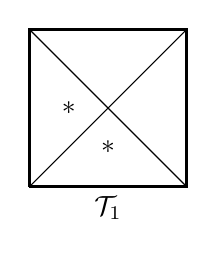
\begin{tikzpicture}[scale=0.5]
\draw (0,4)--(4,0);
\draw (0,0)--(4,4);
\draw[very thick] (0,0)--(4,0)--(4,4)--(0,4)--(0,0);
\node at (2,1) {$\ast$};
\node at (1,2) {$\ast$};
\node[below] at (2,0) {$\mathcal{T}_1$};
\end{tikzpicture}\hfill
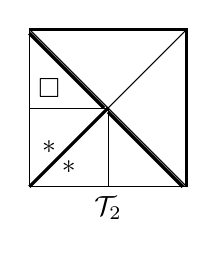
\begin{tikzpicture}[scale=0.5]
\draw (0,0)--(4,0)--(4,4)--(0,4)--(0,0);
\draw (0,4)--(4,0);
\draw (0,0)--(4,4);
\draw (2,0)--(2,2);
\draw (0,2)--(2,2);
\draw[very thick] (4,0)--(4,4)--(0,4);
\draw[very thick] (0,0)--(2,2);
\draw[very thick] (0,3.9)--(1.9,2);
\draw[very thick] (3.9,0)--(2,1.9);
\node at (1,0.5) {$\ast$};
\node at (0.5,1) {$\ast$};
\node at (0.5,2.5) {$\square$};
\node[below] at (2,0) {$\mathcal{T}_2$};
\end{tikzpicture}\hfill
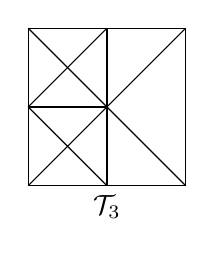
\begin{tikzpicture}[scale=0.5]
\draw (0,0)--(4,0)--(4,4)--(0,4)--(0,0);
\draw (0,4)--(4,0);
\draw (0,0)--(4,4);
\draw (2,0)--(2,2);
\draw (0,2)--(2,2);
\draw (2,0)--(0,2);
\draw (2,2)--(2,4);
\draw (0,2)--(2,4);
\node[below] at (2,0) {$\mathcal{T}_3$};
\end{tikzpicture}
\end{center}

\hfill

\begin{itemize}
  \item Refine by cutting element in two (use newest edge)
  \item Is simple ($\ast$), but may lead to substantial
    non-local changes of the mesh ($\mathcal{T}_2 \to \mathcal{T}_3$,$\square$)
\end{itemize}
\end{frame}

\begin{frame}
\frametitle{Regular Refinement}
\begin{center}
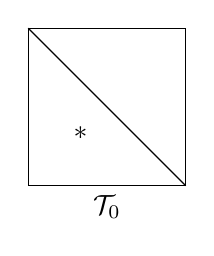
\begin{tikzpicture}[scale=0.5]
\draw (0,0)--(4,0)--(4,4)--(0,4)--(0,0);
\draw (0,4)--(4,0);
\node at (1.33,1.33) {$\ast$};
\node[below] at (2,0) {$\mathcal{T}_0$};
\end{tikzpicture} \hfill
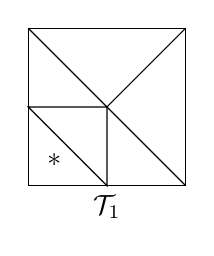
\begin{tikzpicture}[scale=0.5]
\draw (0,0)--(4,0)--(4,4)--(0,4)--(0,0);
\draw (0,4)--(4,0);
\draw (2,0) -- (2,2) -- (0,2) -- cycle;
\draw (2,2)--(4,4);
\node at (0.66,0.66) {$\ast$};
\node[below] at (2,0) {$\mathcal{T}_1$};
\end{tikzpicture} \hfill
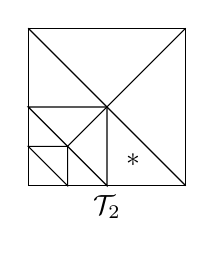
\begin{tikzpicture}[scale=0.5]
\draw (0,0)--(4,0)--(4,4)--(0,4)--(0,0);
\draw (0,4)--(4,0);
\draw (2,0) -- (2,2) -- (0,2) -- cycle;
\draw (2,2)--(4,4);
\draw (1,0) -- (1,1) -- (0,1) -- cycle;
\draw (1,1)--(2,2);
\node at (2.66,0.66) {$\ast$};
\node[below] at (2,0) {$\mathcal{T}_2$};
\end{tikzpicture} \hfill
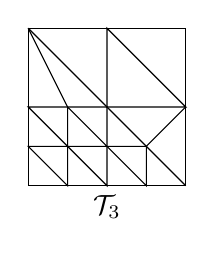
\begin{tikzpicture}[scale=0.5]
\draw (0,0)--(4,0)--(4,4)--(0,4)--(0,0);
\draw (0,4)--(4,0);
\draw (2,0) -- (2,2) -- (0,2) -- cycle;
\draw (1,0) -- (1,1) -- (0,1) -- cycle;
\draw (3,0) -- (3,1) -- (2,1) -- cycle;
\draw (1,1) -- (2,1) -- (1,2) -- cycle;
\draw (2,2) -- (4,2) -- (2,4) -- cycle;
\draw (3,1)--(4,2);
\draw (1,2)--(0,4);
\node[below] at (2,0) {$\mathcal{T}_3$};
\end{tikzpicture}
\end{center}

\hfill

\begin{itemize}
  \item Refine by dividing local mesh width $h_T$ by two,
    produces smaller copies of original element
  \item Requires bisection on the fringe to keep mesh
    conforming
  \item Shape regularity requires removal of bisection
    refinement in subsequent iterations
    ($\mathcal{T}_2 \to \mathcal{T}_3$)
\end{itemize}
\end{frame}

\begin{frame}
\frametitle{Refinement of Quadrilaterals}
\begin{center}
\begin{tikzpicture}[scale=0.5]
\draw (0,0)--(4,0)--(4,4)--(0,4)--(0,0);
\node at (2,2) {$\ast$};
\node[below] at (2,0) {$\mathcal{T}_0$};
\end{tikzpicture} \hfill
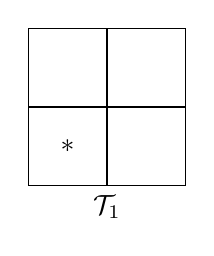
\begin{tikzpicture}[scale=0.5]
\draw (0,0)--(4,0)--(4,4)--(0,4)--(0,0);
\draw (2,0)--(2,4);
\draw (0,2)--(4,2);
\node at (1,1) {$\ast$};
\node[below] at (2,0) {$\mathcal{T}_1$};
\end{tikzpicture} \hfill
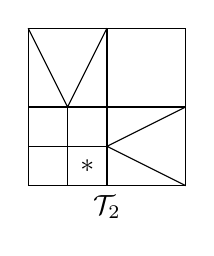
\begin{tikzpicture}[scale=0.5]
\draw (0,0)--(4,0)--(4,4)--(0,4)--(0,0);
\draw (2,0)--(2,4);
\draw (0,2)--(4,2);
\draw (1,0)--(1,2);
\draw (0,1)--(2,1);
\draw (0,4)--(1,2)--(2,4);
\draw (4,0)--(2,1)--(4,2);
\node at (1.5,0.5)  {$\ast$};
\node[below] at (2,0) {$\mathcal{T}_2$};
\end{tikzpicture} \hfill
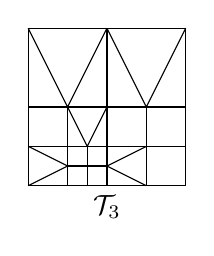
\begin{tikzpicture}[scale=0.5]
\draw (0,0)--(4,0)--(4,4)--(0,4)--(0,0);
\draw (2,0)--(2,4);
\draw (0,2)--(4,2);
\draw (1,0)--(1,2);
\draw (0,1)--(2,1);
\draw (0,4)--(1,2)--(2,4);
\draw (3,0)--(3,2);
\draw (2,1)--(4,1);
\draw (2,4)--(3,2)--(4,4);
\draw (1.5,0)--(1.5,1);
\draw (1,0.5)--(2,0.5);
\draw (0,0)--(1,0.5)--(0,1);
\draw (1,2)--(1.5,1)--(2,2);
\draw (3,0)--(2,0.5)--(3,1);
\node[below] at (2,0) {$\mathcal{T}_3$};
\end{tikzpicture}
\end{center}

\hfill

\begin{itemize}
  \item Regular refinement with conforming closure can be
    used with quadrilaterals
  \item Requires using triangular elements for the closure
  \item Hybrid mesh, no longer one universal reference element
\end{itemize}
\end{frame}

\begin{frame}
\frametitle{Hanging Nodes}
\begin{center}
\begin{tikzpicture}[scale=0.5]
\draw (0,0)--(4,0)--(4,4)--(0,4)--(0,0);
\node at (2,2) {$\ast$};
\node[below] at (2,0) {$\mathcal{T}_0$};
\end{tikzpicture} \hfill
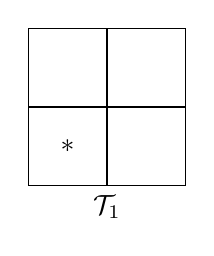
\begin{tikzpicture}[scale=0.5]
\draw (0,0)--(4,0)--(4,4)--(0,4)--(0,0);
\draw (2,0)--(2,4);
\draw (0,2)--(4,2);
\node at (1,1) {$\ast$};
\node[below] at (2,0) {$\mathcal{T}_1$};
\end{tikzpicture} \hfill
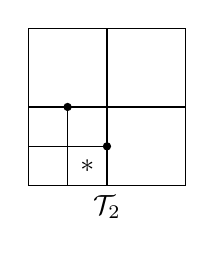
\begin{tikzpicture}[scale=0.5]
\draw (0,0)--(4,0)--(4,4)--(0,4)--(0,0);
\draw (2,0)--(2,4);
\draw (0,2)--(4,2);
\draw (1,0)--(1,2);
\draw (0,1)--(2,1);
\fill(1,2) circle (3pt);
\fill(2,1) circle (3pt);
\node at (1.5,0.5)  {$\ast$};
\node[below] at (2,0) {$\mathcal{T}_2$};
\end{tikzpicture} \hfill
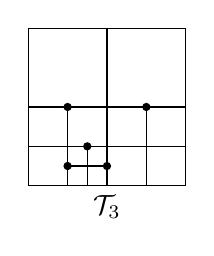
\begin{tikzpicture}[scale=0.5]
\draw (0,0)--(4,0)--(4,4)--(0,4)--(0,0);
\draw (2,0)--(2,4);
\draw (0,2)--(4,2);
\draw (1,0)--(1,2);
\draw (0,1)--(2,1);
\draw (3,0)--(3,2);
\draw (2,1)--(4,1);
\draw (1.5,0)--(1.5,1);
\draw (1,0.5)--(2,0.5);
\fill(1,2) circle (3pt);
\fill(1,0.5) circle (3pt);
\fill(1.5,1) circle (3pt);
\fill(2,0.5) circle (3pt);
\fill(3,2) circle (3pt);
\node[below] at (2,0) {$\mathcal{T}_3$};
\end{tikzpicture}
\end{center}

\hfill

\begin{itemize}
  \item Omitting closure keeps refinement local
  \item Straightforward and can also be used with triangles
  \item Resulting hanging nodes add constraints to the
    finite element space, i.e. algorithmic complexity is
    shifted from mesh generation to assembly procedure
\end{itemize}
\end{frame}


\begin{frame}
\begin{center}
\Large\textbf{Implementation in DUNE/PDELab}
\end{center}
\end{frame}

\begin{frame}
\frametitle{Overview DUNE/PDELab Implementation}
Files involved are:
\begin{enumerate}[1)]
\item File \lstinline{tutorial05.cc} 
\begin{itemize}
\item Includes C++, DUNE and PDELab header files 
\item Contains the \lstinline{main} function
\item Creates a finite element mesh and calls the \lstinline{driver}
\end{itemize}
\item File \lstinline{tutorial05.ini} 
\begin{itemize}
\item Contains parameters controlling the execution
\end{itemize}
\item File \lstinline{driver.hh}
\begin{itemize}
\item Function \lstinline{driver} iteratively solving the finite element problem
  and refining the mesh based on the calculated error estimate
\end{itemize}
\item File \lstinline{nonlinearpoissonfem.hh} 
\begin{itemize}
\item Class \lstinline{NonlinearPoissonFEM} 
realizing the necessary element-local computations for the PDE
\end{itemize}
\item File \lstinline{nonlinearpoissonfemestimator.hh} 
\begin{itemize}
\item Class \lstinline{NonlinearPoissonFEMEstimator} 
realizing the necessary element-local computations for the error estimate
\end{itemize}
\end{enumerate}
Now lets go to the code \ldots
\end{frame}

\end{document}

